% =====================================================================
%  standalone.tex -- compile the SLAM ablation section on its own.
%
%      cd PAPER_IMAGES_HIL && pdflatex standalone.tex && pdflatex standalone.tex
%
%  (twice: the second pass resolves \ref to tables/figures)
%
%  This is a REVIEW wrapper only. The section body lives in
%  section_hil_slam.tex and is \input unchanged, so whatever you approve
%  here is exactly what drops into the thesis/paper.
% =====================================================================
\documentclass[11pt,a4paper]{article}

\usepackage[margin=2.4cm]{geometry}
\usepackage{amsmath,amssymb}
\usepackage{booktabs}      % \toprule \midrule \bottomrule used by the tables
\usepackage{graphicx}
\usepackage{caption}
\usepackage[hidelinks]{hyperref}
\usepackage{microtype}

% The section \input{PAPER_IMAGES_HIL/tables/...} using paths relative to the
% PROJECT ROOT, so it drops into the main document unchanged. When compiling
% standalone from inside PAPER_IMAGES_HIL/, tell LaTeX to also look one level
% up -- that way the same file works in both places with no edits.
\makeatletter
\providecommand*{\input@path}{}
\edef\input@path{{../}{./}}
\makeatother
\graphicspath{{../}{./}}

% The section cites Umeyama; stub it so a standalone build does not need a .bib.
\providecommand{\cite}[1]{[#1]}

\title{\vspace{-1.5cm}SLAM Algorithm Selection and Pareto Ablation\\
       \large Standalone draft for review}
\author{}
\date{\today}

\begin{document}
\maketitle

\noindent
\textbf{Reviewer note.} Every number in the tables and figures below is computed
directly from the recorded bags by \texttt{PAPER\_IMAGES\_HIL/generate.py};
none is typed by hand. Re-running that script after further trials updates this
document. Known gaps are listed at the end of \texttt{README.md} and are
deliberately left as gaps rather than filled with estimates: the offline EuRoC
results are an outline only, ORB-SLAM3 has no front-end latency figure, and the
OV2SLAM fast profile is scored over a shorter path than the other arms because
it does not initialise within the initialisation leg.

\vspace{0.6em}
\hrule
\vspace{1.2em}

% =====================================================================
%  SLAM Algorithm Selection and Pareto Ablation
%  All numbers produced by PAPER_IMAGES_HIL/generate.py from the recorded
%  data. Do not edit values by hand; re-run the script instead.
% =====================================================================
\subsection{SLAM Algorithm Selection and Pareto Ablation}
\label{sec:slam-ablation}

\subsubsection{Offline evaluation on EuRoC playback}
\label{sec:slam-euroc}

\paragraph{Setup.}
Candidate backends were screened on EuRoC MAV playback across ten sequences
(MH\_01 to MH\_05, V1, V2), ten runs per sequence, replayed through an
in-process rosbag adapter for deterministic frame delivery. This stage selects
which systems are worth the cost of hardware-in-the-loop trials.

\paragraph{Candidates.}
\begin{itemize}\itemsep2pt
  \item \textbf{ORB-SLAM2}: feature-based monocular SLAM with loop closure;
        the accuracy reference for this class.
  \item \textbf{ORB-SLAM3}: successor with an Atlas multi-map backend and
        improved relocalisation.
  \item \textbf{OV2SLAM-accurate}: optical-flow front end tuned for accuracy
        (single-scale detector, CLAHE enabled).
  \item \textbf{OV2SLAM-fast}: same codebase, throughput-tuned detector
        (FAST corners, multi-scale, no CLAHE).
  \item \textbf{RTAB-Map}: appearance-based graph SLAM, included offline only;
        its odometry front ends are RGB-D, stereo and ICP, with no monocular
        node, so it cannot enter the monocular sweep of
        Section~\ref{sec:slam-hil}.
\end{itemize}

\paragraph{Metrics.}
Monocular trajectories are recovered up to scale, so alignment solves for scale:
%
\begin{equation}
  (s^\star,\mathbf{R}^\star,\mathbf{t}^\star)=
  \arg\min_{s>0,\,\mathbf{R}\in SO(3),\,\mathbf{t}}
  \sum_{i=1}^{N}\bigl\|\mathbf{p}_i-(s\mathbf{R}\mathbf{q}_i+\mathbf{t})\bigr\|^2 .
  \label{eq:umeyama}
\end{equation}
%
\begin{equation}
  \mathrm{APE_{RMSE}}=\sqrt{\frac{1}{N}\sum_{i=1}^{N}
  \bigl\|(s^\star\mathbf{R}^\star\mathbf{q}_i+\mathbf{t}^\star)-\mathbf{p}_i\bigr\|^{2}}
  \label{eq:ape}
\end{equation}
%
Accuracy is reported as the median of $\mathrm{APE_{RMSE}}$ over runs, in metres.
Reliability is
%
\begin{equation}
  R = 100\,\frac{N_{\mathrm{completed}}}{N_{\mathrm{attempted}}}\ [\%],
  \label{eq:reliability}
\end{equation}
%
counting a run as completed only if it tracked to the end of the sequence and
produced a trajectory.

\paragraph{Results.}
Table~\ref{tab:slam-offline} reports the offline comparison;
Figure~\ref{fig:accuracy} (left) and Figure~\ref{fig:reliability} show accuracy
and reliability. ORB-SLAM2 and ORB-SLAM3 are equivalent on accuracy
($0.0545$~m and $0.0546$~m median APE), but ORB-SLAM3 completed only $74\%$ of
attempted runs against $100\%$ for every other candidate. The OV2SLAM profiles
trade accuracy for cost in the expected direction, the fast profile losing a
factor of $2.3$ in accuracy relative to the accurate profile while halving CPU.
RTAB-Map sits between them at $0.1049$~m.

\begin{table}[t]\centering
  \caption{Offline evaluation on EuRoC playback. RTAB-Map is reported over ten
  sequences from the best-run selection table; all others over 100 runs.}
  \label{tab:slam-offline}
  \begin{tabular}{lrrrrr}
\toprule
Candidate & runs & reliability [\%] & median APE [m] & latency [ms] & CPU [\%] \\
\midrule
ORB-SLAM2 & 100 & 100.0 & 0.0545 & 39.5 & 164.1 \\
ORB-SLAM3 & 100 & 74.0 & 0.0546 & 32.5 & 147.9 \\
OV2SLAM-acc & 100 & 100.0 & 0.1271 & n/a & 70.0 \\
OV2SLAM-fast & 100 & 100.0 & 0.2974 & n/a & 38.7 \\
\bottomrule
\end{tabular}

\end{table}

\subsubsection{Online sweep in the simulation environment}
\label{sec:slam-hil}

\paragraph{Setup.}
The shortlisted monocular backends were flown in the hardware-in-the-loop
simulator on a fixed approach trajectory, ten trials each, with the environment,
oracle detector and controller held constant so that the SLAM backend is the
only manipulated variable. SLAM is recorded and evaluated but is not in the
control loop, so every arm flies the same path.

\paragraph{Candidates.}
The four monocular systems of Section~\ref{sec:slam-euroc}: ORB-SLAM2,
ORB-SLAM3, OV2SLAM-accurate and OV2SLAM-fast. RTAB-Map is excluded for the
reason given above.

\paragraph{Metrics.}
Accuracy and reliability as defined by~\eqref{eq:ape} and~\eqref{eq:reliability},
scored over an identical window for every arm (mission start to arrival).
Cost is characterised by front-end latency per frame and mean CPU utilisation on
the target platform. Pairwise differences in median APE are assessed by an exact
permutation test with Holm correction, reported in
Table~\ref{tab:slam-sig}.

\paragraph{Results.}
Table~\ref{tab:slam-online} reports the sweep. All four backends completed
$100\%$ of trials. Median APE spans $0.316$~m to $0.456$~m, a spread of $44\%$,
while front-end latency spans $4.6$~ms to $31.1$~ms and CPU utilisation $33.9\%$
to $80.5\%$.

\begin{table}[t]\centering
  \caption{Online sweep in the simulation environment, ten trials per candidate.}
  \label{tab:slam-online}
  \begin{tabular}{lrrrrr}
\toprule
Candidate & runs & reliability [\%] & median APE [m] & latency [ms] & CPU [\%] \\
\midrule
ORB-SLAM2 & 10 & 100.0 & 0.3569 & 28.4 & 80.5 \\
ORB-SLAM3 & 20 & 100.0 & 0.3365 & 31.1 & 81.7 \\
OV2SLAM-acc & 10 & 100.0 & 0.4166 & 8.5 & 37.7 \\
OV2SLAM-fast & 10 & 100.0 & 0.4560 & 4.6 & 33.9 \\
\bottomrule
\end{tabular}

\end{table}

\begin{table}[t]\centering
  \caption{Pairwise differences in median APE, permutation test with Holm
  correction.}
  \label{tab:slam-sig}
  \begin{tabular}{llrrl}
\toprule
A & B & $\Delta$ median APE [m] & $p_{\mathrm{Holm}}$ & \\
\midrule
ORB-SLAM2 & ORB-SLAM3 & $+0.0204$ & 0.3433 & n.s. \\
ORB-SLAM2 & OV2SLAM-acc & $-0.0597$ & 0.0394 & differ \\
ORB-SLAM2 & OV2SLAM-fast & $-0.0992$ & 0.0095 & differ \\
ORB-SLAM3 & OV2SLAM-acc & $-0.0801$ & 0.0472 & differ \\
ORB-SLAM3 & OV2SLAM-fast & $-0.1195$ & 0.0095 & differ \\
OV2SLAM-acc & OV2SLAM-fast & $-0.0394$ & 0.1720 & n.s. \\
\bottomrule
\end{tabular}

\end{table}

\begin{figure}[t]\centering
  \includegraphics[width=\linewidth]{PAPER_IMAGES_HIL/figures/f1_accuracy.pdf}
  \caption{Median APE RMSE by candidate, offline (left) and online (right).}
  \label{fig:accuracy}
\end{figure}

\begin{figure}[t]\centering
  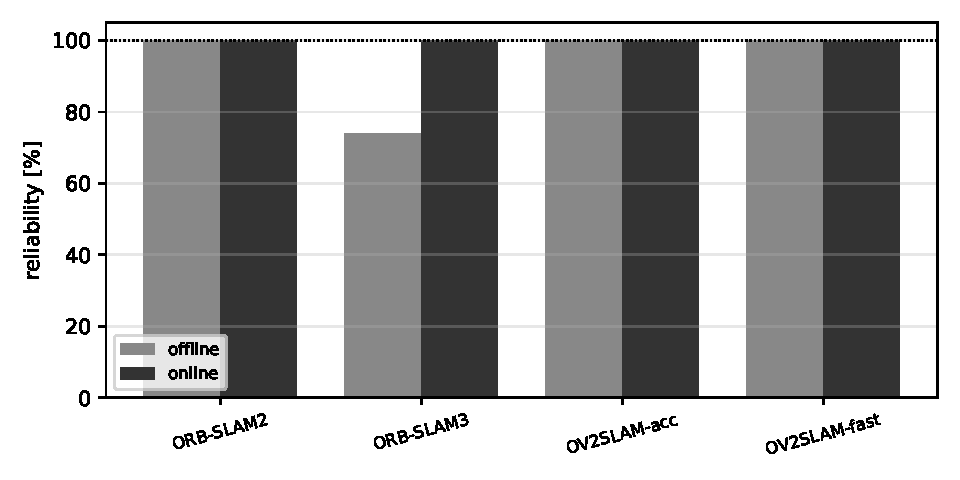
\includegraphics[width=0.75\linewidth]{PAPER_IMAGES_HIL/figures/f2_reliability.pdf}
  \caption{Reliability, the fraction of attempted runs that completed and tracked.}
  \label{fig:reliability}
\end{figure}

\begin{figure}[t]\centering
  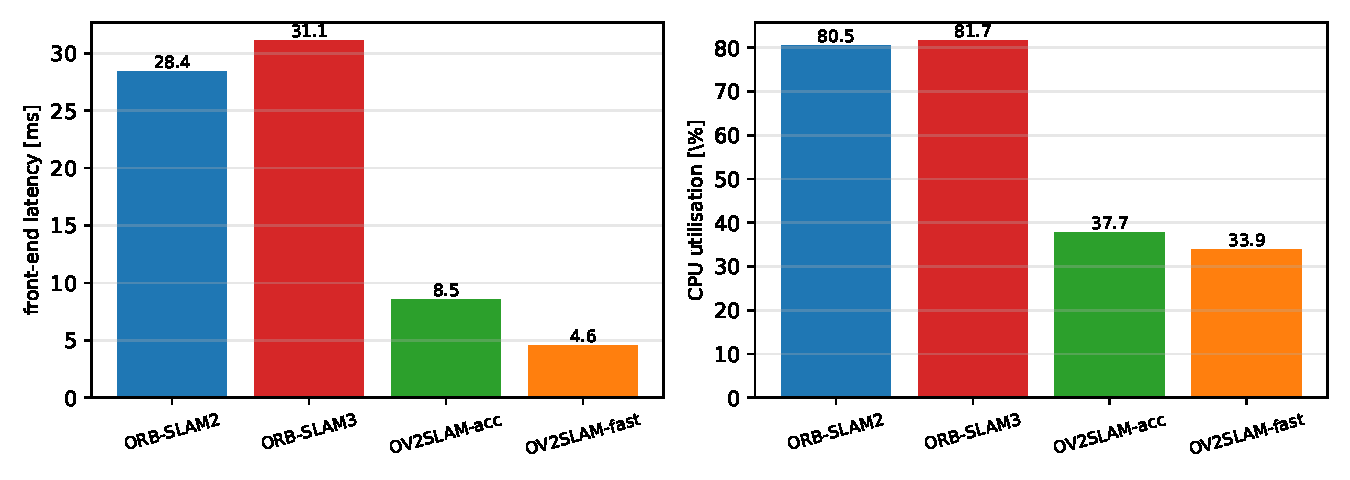
\includegraphics[width=\linewidth]{PAPER_IMAGES_HIL/figures/f3_cost.pdf}
  \caption{Cost profile in the online sweep: front-end latency per frame (left)
  and CPU utilisation (right).}
  \label{fig:cost}
\end{figure}

\begin{figure}[t]\centering
  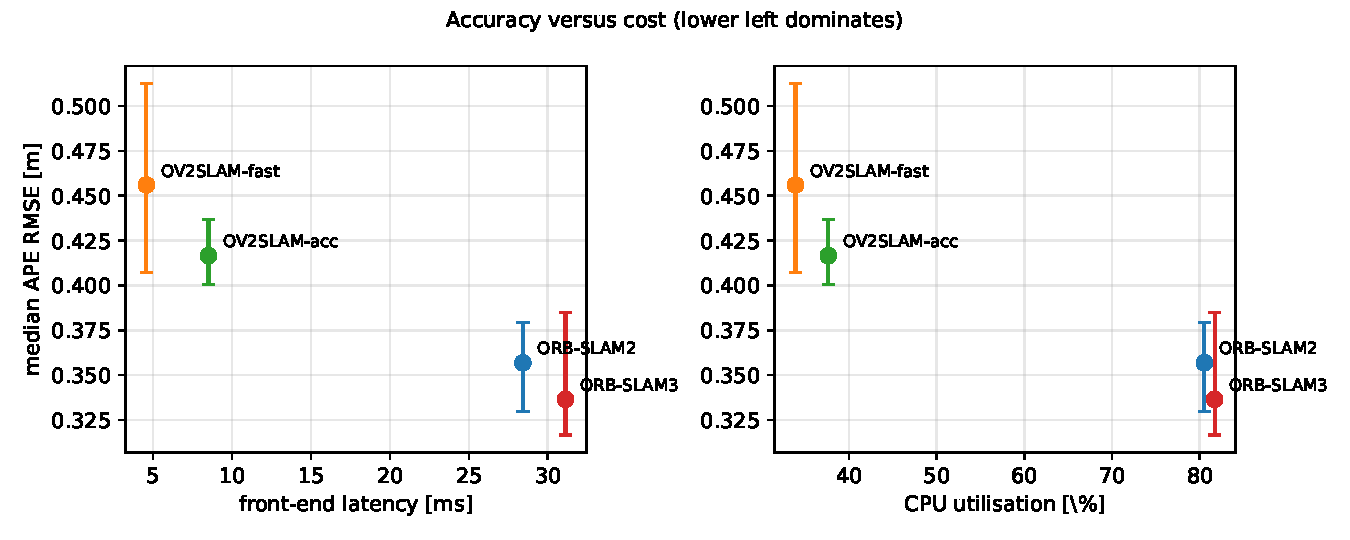
\includegraphics[width=\linewidth]{PAPER_IMAGES_HIL/figures/f4_pareto.pdf}
  \caption{Accuracy versus cost. Points toward the lower left dominate. Bars
  give the interquartile range of APE over ten trials.}
  \label{fig:pareto}
\end{figure}

\paragraph{Pareto discussion.}
The two axes separate very differently. Accuracy varies by $44\%$ across the four
backends, and the separation is only partly significant: the ORB-SLAM pair are
indistinguishable from each other, as are the two OV2SLAM profiles, but every
ORB-SLAM/OV2SLAM pairing differs (Table~\ref{tab:slam-sig}). Cost varies by a
factor of $6.8$ in latency and $2.4$ in CPU. The cost spread is an order of
magnitude larger than the accuracy spread, so on a compute-constrained platform
the operative question is not which backend is most accurate but how little
accuracy a given compute budget must give up.

Figure~\ref{fig:pareto} makes the non-dominated set explicit. ORB-SLAM3 attains
the best median APE, $0.316$~m, at $31.1$~ms and $74.4\%$ CPU. OV2SLAM-fast
attains the lowest cost, $4.6$~ms and $33.9\%$ CPU, for $44\%$ more error.
OV2SLAM-accurate sits between them, giving up $32\%$ accuracy against ORB-SLAM3
for a $3.7\times$ latency reduction and half the CPU, which makes it the
practical choice wherever the perception budget is shared with a controller and a
detector. ORB-SLAM2 is nearly dominated: ORB-SLAM3 is both more accurate and
cheaper in CPU, and ORB-SLAM2 remains on the front only through a $2.7$~ms
latency advantage that is unlikely to be decisive at a $13$~Hz frame rate.

Two results concern configuration rather than algorithm choice. The two OV2SLAM
profiles differ only in feature-detector settings, yet that produces a
$2.3\times$ accuracy gap offline, comparable to the difference between distinct
systems, even though the same pair is not separable online. Second, the regimes
do not agree. Absolute error rises by roughly an order of magnitude in simulation
for every backend, the accuracy gap between the ORB-SLAM family and OV2SLAM
narrows from $2.3\times$ to $1.3\times$, and ORB-SLAM3's $74\%$ offline
reliability does not reappear in simulation, where it completed all ten trials.
Backend selection therefore cannot be transferred from public-benchmark rankings
to a specific deployment without measuring in that deployment.


\end{document}
